\chapter{Graded membership strategy}
\label{s:graded-membership-strategy}
\is{language strategy!for colour!graded membership strategy}
\is{graded membership strategy|see{language strategy}}

Colour categories are assumed to be prototypical in nature
\citep{rosch73natural}, which implies that some colour samples are
better examples of a category than others. Some languages allow the
users to mark how well a particular sample represents the
prototype. In English this marking is optional and achieved through
the adverb \textit{very} and the modifying \textit{-ish} suffix, such as in the
expression \textit{greenish}. In Russian, the suffix \textit{-ato} indicates a
similar meaning \citep{safuanova07russian}. In other languages, such
as Tarahumara, an indigenous language spoken in Northern Mexico, this
marking is obligatory. This language has an elaborate system of
modifiers that distinguishes three levels of membership: \textit{-kame}
which could be translated as \textit{very}, \textit{-name} which could be
glossed as \textit{somewhat} and \textit{-nanti} for the lowest degree of
membership. An example of how this system is used for the Turahumara
colour category for red: \textit{Sit\'a-} is shown in Figure
\ref{f:gms-burgress-tarahumara} \citep{burgress83tarahumara}.

\begin{figure}[htbp]
  \begin{center}
   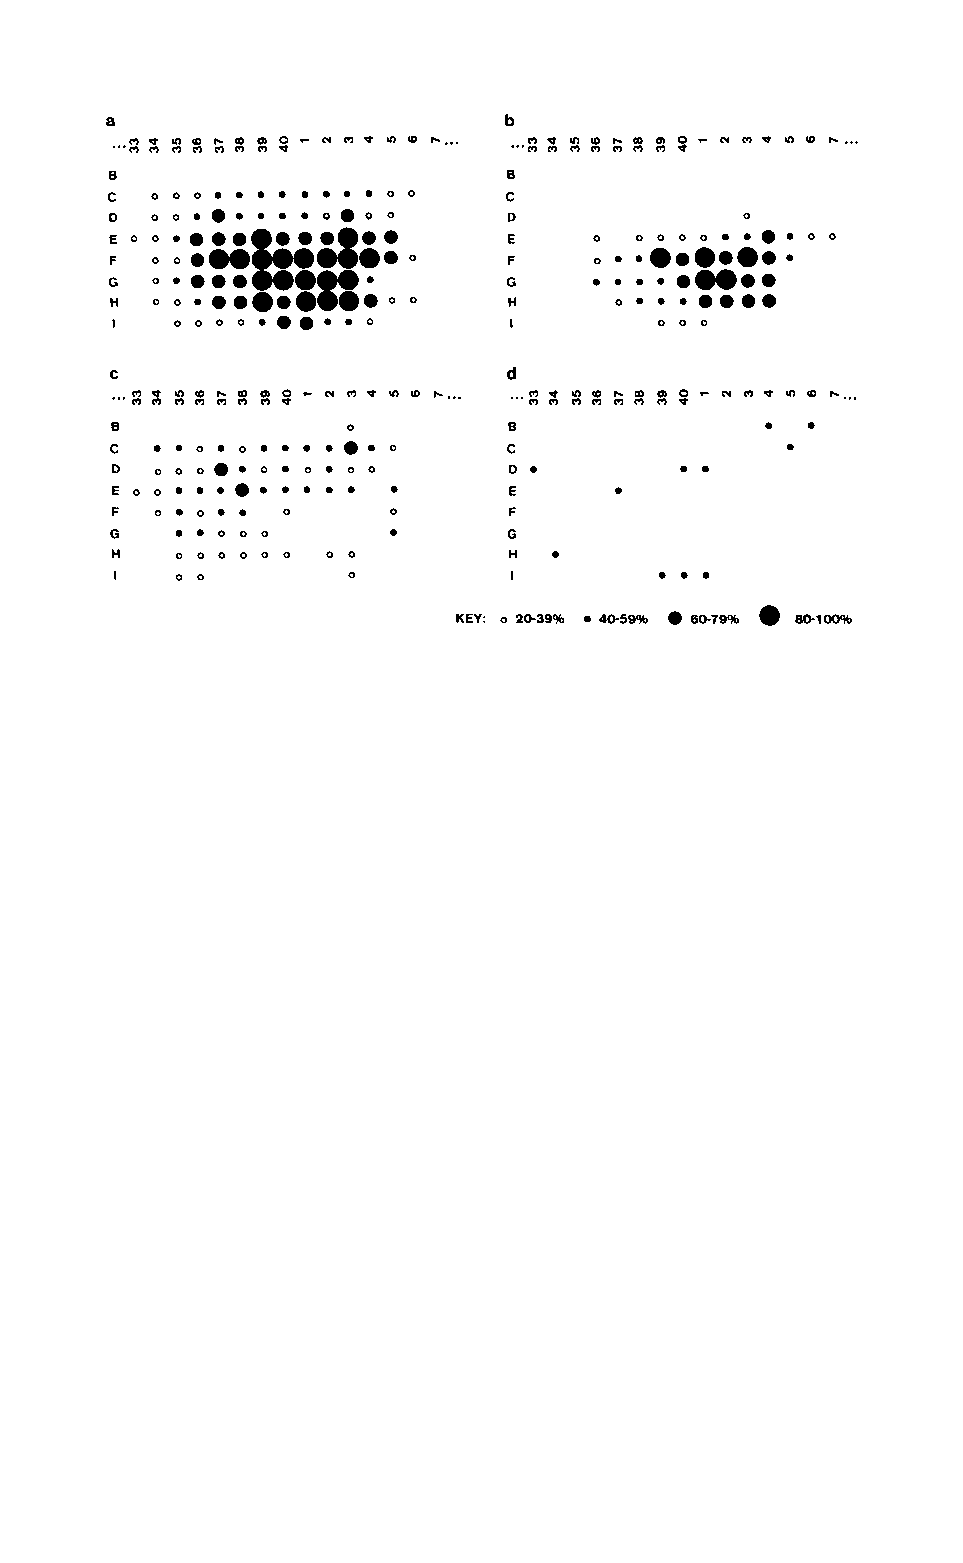
\includegraphics[width=\textwidth]{./graded-membership/figures/burgress-tarahumara.pdf}
   \caption[The use of modifiers in Tarahumara]{The use of modifiers
     to express graded membership in Tarahumara shown on the Munsell
     array. The bigger the circle, the more it represents a
     particular colour expression. (a) aggregate of all expressions
     using the \textit{Sit\'a} root (b) \textit{Sit\'akame} (`very red') (c)
     \textit{Sit\'aname} (`somewhat red') (d) \textit{Sit\'ananti} (`only slightly
     red'). Note how each modifier specifies a region that is further
     removed from the prototypical colour of \textit{Sit\'a}. Figure from
     \cite{burgress83tarahumara}.}
    \label{f:gms-burgress-tarahumara}
  \end{center}
\end{figure}

In this chapter, I will propose a compositional semantic template that
is capable of modelling these observations. I will also introduce the
grammatical syntactic templates that allow agents to express this
strategy in language. I will use Tarahumara as the main guiding
example.

\section{Related research}
\label{s:gms-related-research}

Although most models within artificial language evolution and colour
naming models represent the graded nature of membership of a colour
sample to a colour category, almost none of them deploy syntax to
express this membership. One exception is the colour naming model of
\citeauthor{mojsilovic02method}, which includes names for modifiers
and different lightness values \citep{mojsilovic02method,
  mojsilovic05computational}. The semantics of this model, however, is
quite limited as each compositional colour name is stored as a
different prototype based on a dictionary of colour names compiled by
the National Bureau of Standards \citep{kelly53icss}. It is unclear
how this model could be extended to allow for creative language use,
for example when names are not explicitly listed in the dictionary.

\section{Semantic template}
\label{s:gms-semantic-template}
\is{semantic template!for graded membership strategy}

Degree modifiers make the degree of membership of a particular entity
in the world to a category in the ontology of an agent explicit in
language. They split the continuous domain of membership into more or
less discrete categories. In order to propose semantics that capture
these observations, I need to make two choices: how the membership
function is computed and how the categorisation process based on this
membership function is implemented.

The membership function corresponds to the similarity function
introduced in Section \ref{s:bcs-categorisation}. The similarity of
the colour of an entity to a colour category maps directly on the
membership function: the more similar the colour of entity to the
prototype of the category, the higher the membership. The maximum
value of the membership function is one (when the colour of the entity
is exactly equal to the prototype of the category) and approaches zero
when they are very dissimilar.

The \textsc{membership categories} are implemented as prototypical
categories. Each category has a prototypical value of the membership
and classification is organised following a standard nearest-neighbour
algorithm. Each entity is assigned to the membership category that is
most similar to it. Other approaches, such as discrimination trees
\citep{steels96perceptually}, could have been chosen, but the
prototype theory is sufficient to cover the main principles of the
graded membership strategy.

This approach results in the definition of absolute ranges between a
colour sample and colour category due to the properties of the
membership function and how the membership categorisation process is
organised. The membership function is only dependent on the category
that is most similar to the sample and the membership categories are
defined as prototypical values of this membership function. As a net
result, a membership category defines an absolute range in distance
between the colour sample and the colour category. A schematic
representation of this approach is provided in Figure
\ref{f:gms-semantics-schematic}.

\begin{figure}[htbp]
  \centering
  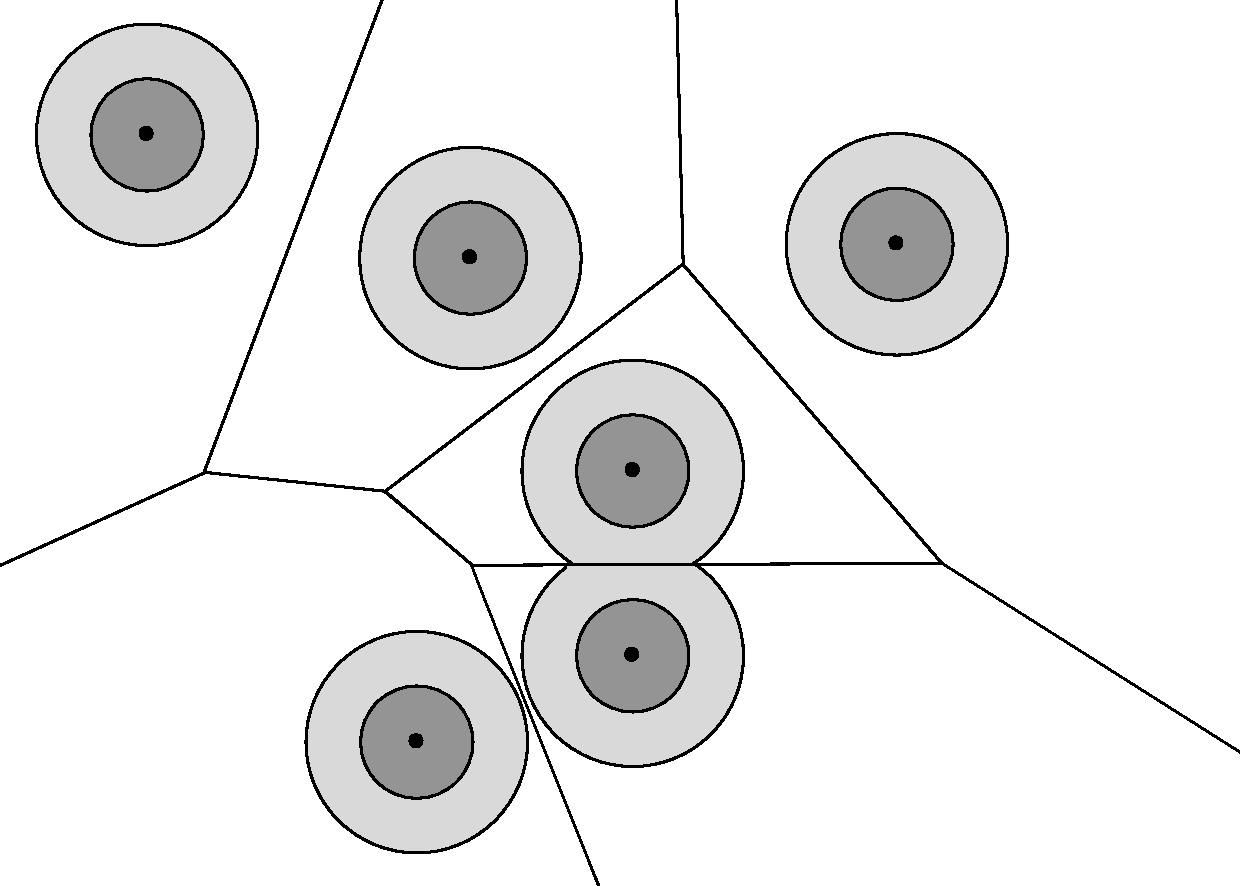
\includegraphics[width=.5\textwidth]{./graded-membership/figures/semantics-schematic.pdf}
  \caption[Schematic representation of the semantics of the graded
  membership strategy]{Schematic representation of the semantics of
    the graded membership. The categorisation based on colour
    categories results in a Voronoi tessellation of the conceptual
    space. The membership categories (marked in different shades of
    grey) define a fixed range starting from the prototype of the
    category.}
  \label{f:gms-semantics-schematic}
\end{figure}

The semantics of the graded membership strategy can be
summarised as follows: first the entities are categorised as in the
basic colour strategy. This process stores membership
information in the entities as a side-effect. Unlike the basic
  colour strategy, not just the best member will be selected from
this set, but the resulting set will be categorised again based on the
membership information stored in the entities. This second
categorisation process changes the activation stored in the
entities. Selection will be based on this activation.

\subsection{Profiling and categorisation based on colour}

The categorisation process is similar to the one introduced for the
basic colour strategy, except that this categorisation process
is now more strict. Even in interpretation, it assigns each entity to
the nearest known colour category. This is identical to the
categorisation during conceptualisation.

This modification is based on the observation that whenever the
graded membership strategy is used, the base category will be
the category that is the most similar to the named sample. For
example, a sample that is named \textit{greenish} is still more similar to
the prototype for green than to the prototype of brown.

Although strict interpretation is known to decrease the expected
communicative success when categories are not aligned between
individual language users \citep{belpaeme07language}, it ensures the
categorisation process applied by the speaker and hearer are
symmetrical. This is especially useful when processes become dependent
on each other. Asymmetrical processing might be another source of
potential communicative failures.

\subsection{Categorisation based on membership}

Each membership category is represented by its most prototypical
membership value. The membership value of each entity is compared to
the membership value stored in the category. Each entity is assigned
to the membership category that is most similar to it. More than one
entity can be categorised as the same category. This categorisation
process changes the activation in the entities.

\subsection{Selection based on activation}

This second categorisation process based on membership changes the
activation stored in the entities. The entity with the highest
activation will be selected as the outcome of the complete process.

\subsection{Semantic constraint network}

The semantic constraint network for the graded membership
  strategy is shown in Figure \ref{f:gms-semantic-program}. The
\textsc{Equal-to-Context} and \textsc{Profile-Colour-Dimensions}
primitives are the same ones as introduced before. The
\textsc{Filter-by-Colour} primitive is similar to the
\textsc{Filter-by-Colour-Lenient} except that during interpretation it
applies a strict categorisation as well. The
\textsc{Filter-by-Membership} categorises the resulting sets based on
the membership information stored by the \textsc{Filter-by-Colour}
primitive. Finally, \textsc{Select-Most-Activated} selects the entity
with the highest activation.

\begin{figure}[htbp]
  \centering
  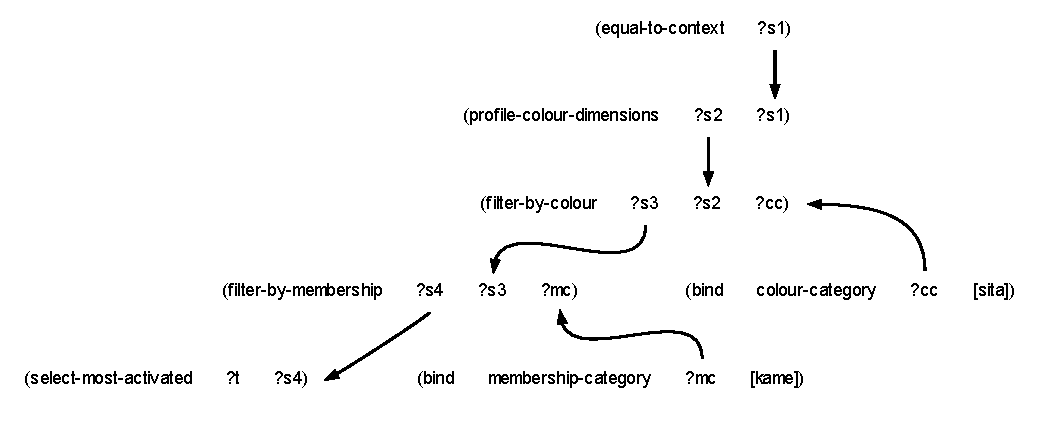
\includegraphics[width=\textwidth]{./graded-membership/figures/semantic-program.pdf}
  \caption[The semantic constraint network for the graded membership
  strategy]{The semantic constraint network for the graded membership
    strategy, which is similar to the one of the basic colour
    strategy. The \textsc{Filter-By-Membership} now categorises the
    resulting sets further. \textsc{Select-Most-Activated} selects the
    entity with the highest activation.}
  \label{f:gms-semantic-program}
\end{figure}

\subsection{Semantic primitives}

\definition{Semantic primitive}{Filter-by-Colour}

\begin{explanation}{description}
  Categorises each entity in a source set as the most similar colour
  category known to the agent. The membership of each entity is set to
  be the the similarity to the category it belongs to.
\end{explanation}

\begin{explanation}{slots}
  \verb+?filtered-set+ (of type entity-set) \\
  \verb+?source-set+ (of type entity-set) \\
  \verb+?colour-category+ (of type colour-category)
\end{explanation}

\begin{explanation}{revision specs}
  \verb+?source-set+: categorises each entity of source set and
  returns pairwise bindings for the remaining slots; categories
  to which no entities are assigned, are ignored \\
  \verb+?source-set ?category+: computes the categorisation of the
  source set based on all colour categories known to the agent and
  when the resulting set for the provided colour category is not
  empty, it gets bound to \verb+?filtered-set+
\end{explanation}

\definition{Semantic primitive}{Filter-by-Membership}

\begin{explanation}{description}
  Categorises each entity in a source set as the most similar
  membership category known to the agent.
\end{explanation}

\begin{explanation}{arguments}
  \verb+?filtered-set+ (of type entity-set) \\
  \verb+?source-set+ (of type entity-set) \\
  \verb+?membership-category+ (of type membership-category)
\end{explanation}

\begin{explanation}{revision specs}
  \verb+?source-set+: categorises each entity in the source set as one
  of the known membership categories and returns pair-wise bindings
  for \verb+membership-category+ and \verb+?filtered-set+ \\
  \verb+?source-set ?membership-category+: computes the categorisation
  of the source set based on all membership categories known to the
  agent and when the resulting set for the provided membership category
  is not empty, it gets bound to \verb+?filtered-set+
\end{explanation}

% \definition{Semantic Primitive}{Select-Unique-Element}

% \begin{explanation}{description}
%   Checks whether an entity set contains only one element and binds it
%   to the other slot.
% \end{explanation}

% \begin{explanation}{slots}
%   \verb+?entity+ (of type colour-entity) \\
%   \verb+?entity-set+ (of type entity-set)
% \end{explanation}

% \begin{explanation}{revision specs}
%   \verb+?entity-set+: when the entity-set is a singleton, binds
%   \verb+?entity+ to its sole member
% \end{explanation}

\subsection{Alternative approaches to semantics}

Several alternative approaches to the proposed semantics exist. One
alternative that has been used in previous models is to model basic
colour categories as one or more multidimensional ``normalised''
Gaussian functions \citep{lammens94computational,
  steels05coordinating}. The similarity measure between a colour
category and a colour sample is weighted by the inverse of the
standard deviation in each dimension. This distance measure is also
known as the Mahalanobis distance.

It might be tempting to model graded membership by modifying the
standard deviation of a category: intensifiers such as \textit{very} could
be implemented as decreasing the standard deviation and diminutives
like \textit{slightly}, could increase the standard deviation. This
corresponds to the idea that intensified categories should be
interpreted more strictly, which is reflected by a lower standard
deviation. This however leads to the unwanted outcome that the
diminutive will always be preferred among the three variants
(intensifier, diminutive and unmodified) as it results in the lowest
distance and hence the highest similarity to a particular colour
sample. This is due to the Mahalanobis measure which divides the
distance in each dimension by its standard deviation. The higher the
standard deviation, the lower the distance. A different similarity or
distance function would be needed to extend this approach to
modifiers.

Another approach that has often been pursued for modelling categories
is based on the fuzzy set theory \citep{kay78linguistic,
  benavente08parametric}. Some features of language, including
modifiers, have been studied using this approach
\citep{hersh76fuzzy}. These studies suggested that the probability of
the membership of an intensified category is a power of the membership
of the unintensified category. This again reflects the intuitive idea
that membership to an intensified category should decrease faster than
membership to the original category, but fails to account for why
intensified categories should be favoured over orginal categories for
the best members of the fuzzy set.

\section{Syntactic templates}
\label{s:gms-syntactic-templates}

The templates to express this network in language are in general
similar to the one used for the basic colour strategy in
Section \ref{s:bcs-syntactic-templates}: the semantic network is
divided in three layers of units: (a) entity units containing the
semantic entities, (b) functional units which make direct use of such
a semantic entity and (c) contextual units which contain any remaining
operations of the semantic constraint network that do not make direct
use of any semantic entity. The main difference is that in order to
express both the basic colour strategy and the graded
  membership strategy, an additional template can be used to allow
the re-use of the contextual rule introduced for the basic colour
strategy.

The linguistic structure for \textit{sita-kame} is shown in Figure
\ref{f:gms-linguistic-structure}. Besides introducing the colour
category for \textit{sita}, the lexicon rules now also introduce the
membership category for \textit{kame}. Functional rules take care of the
\textsc{Filter-by-Colour} and \textsc{Filter-by-Membership}
primitives. All other parts of the semantic network are grouped in a
contextual rule, which also ensures that the two functional primitives are
linked into the other primitives of the network.

\begin{figure}[htbp]
  \centering
  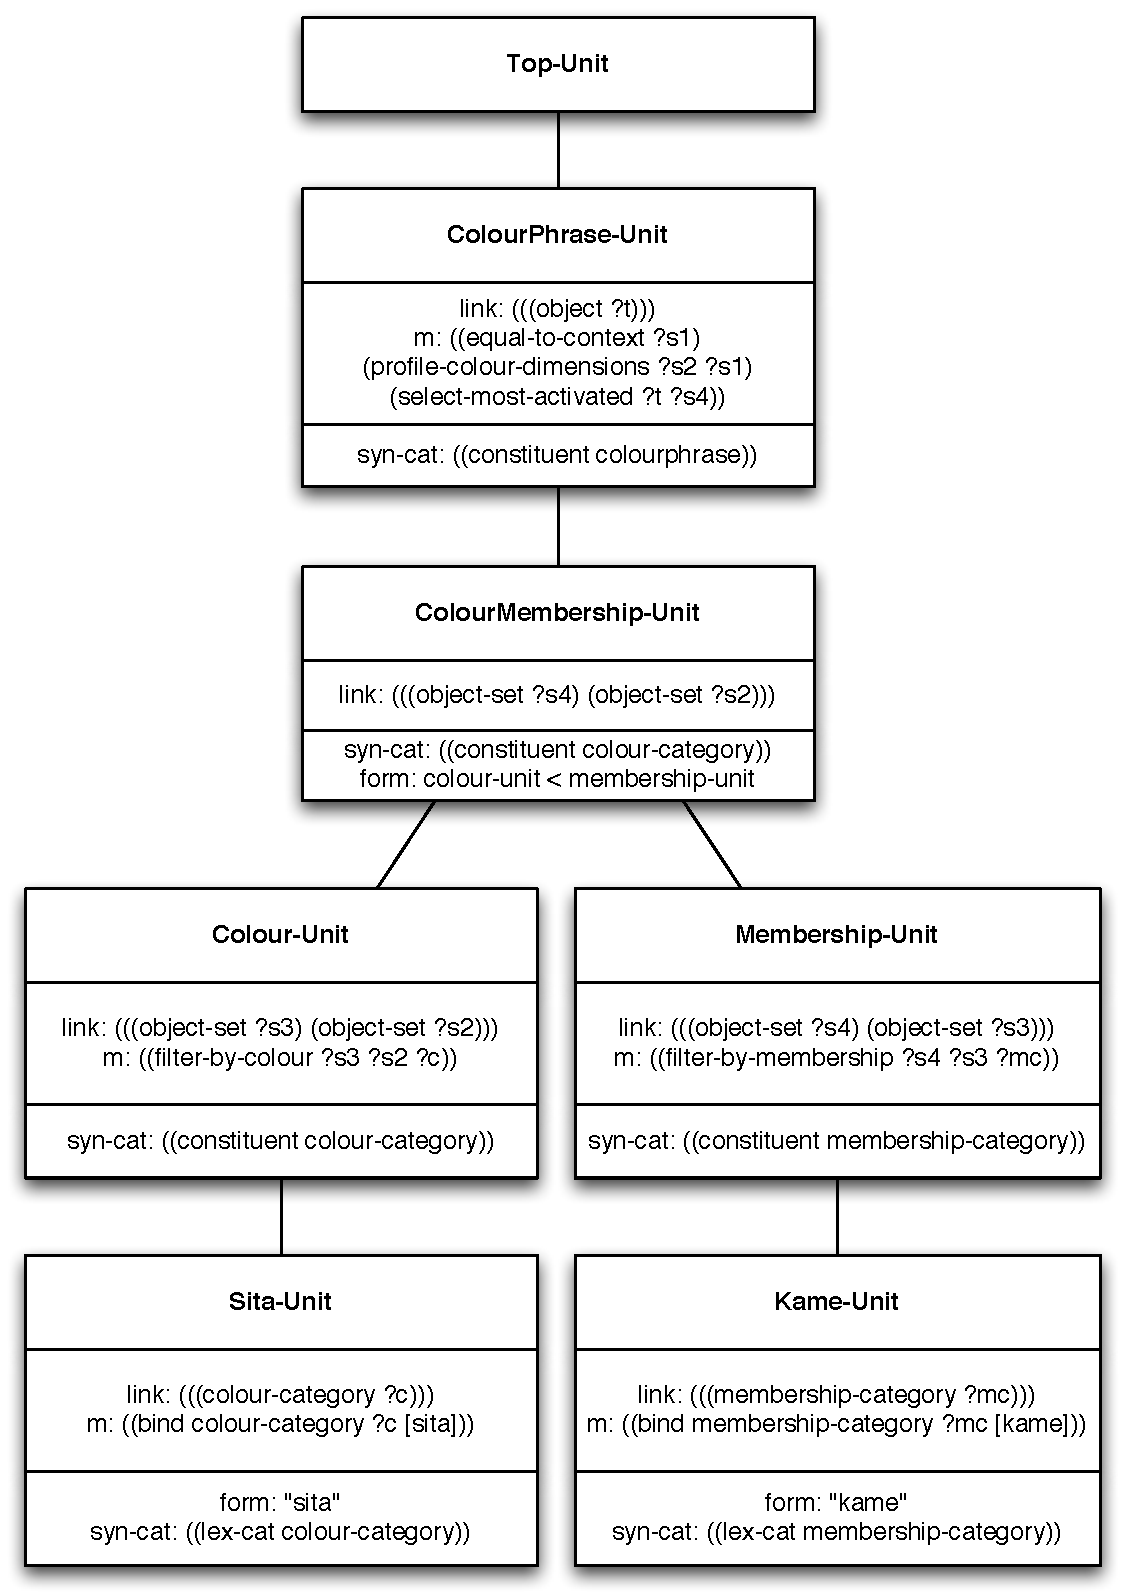
\includegraphics[width=.85\textwidth]{./graded-membership/figures/linguistic-structure.pdf}
  \caption[Linguistic structure for graded membership
  strategy]{Linguistic structure for graded membership strategy. Both
    semantic and syntactic poles are shown in the same
    structure. Semantic information is shown in the top part of each
    unit, the syntactic information in the bottom part of each
    unit. The structure consists of four layers: one for the semantic
    entities, one for the functional primitives and the top one
    represents the contextual rule introduced in the previous
    chapter. The additional ColourMembership-Unit is introduced by a
    rule based on Syntactic template 2.}
  \label{f:gms-linguistic-structure}
\end{figure}

\subsection{Syntactic template 1.1: Semantic entities}
\is{syntactic template!for semantic entities}

The entity rules for membership categories are very similar to the one
I introduced in the previous chapter for colour categories. During
parsing it will introduce the membership category. In production, it
will introduce the string that is associated with this category. In
both modes a new unit is introduced that encapsulates this
information. On the semantic side, the \emph{link} feature
will allow
other rules to incorporate the membership category in the semantic
network during parsing.

\footnotesize
\ltitle{Entity rule for kame}
\begin{lstlisting}
((?top-unit
  (tag ?meaning 
       (meaning ((bind membership-category ?c [kame])))))
 ((J ?kame-unit ?top-unit)
  ?meaning
  (link (((membership-category ?mc))))))
<-->
((?top-unit
  (tag ?form 
       (form ((string ?yellow-unit "kame")))))
 ((J ?kame-unit ?top-unit)
  ?form
  (syn-cat ((lex-cat membership-category)))))
\end{lstlisting}
\normalsize

\subsection{Syntactic template 1.2: Functional primitives}
\is{syntactic template!for functional primitives}

The functional rules for \textsc{Filter-by-Colour} and
\textsc{Filter-by-Membership} are similar to the functional rule for 
\textsc{Filter-by-Colour-Lenient} in the previous chapter. An example
of such a rule for \textsc{Filter-by-Membership} is shown below.

\footnotesize
\ltitle{Functional rule for Filter-by-Membership}
\begin{lstlisting}
((?top-unit
  (sem-subunits (?membership-category-unit)) 
  (tag ?meaning
       (meaning ((filter-by-membership ?s4 ?s3 ?mc)))))
 (?membership-category-unit 
  (link (((membership-category ?c)))))
 ((J ?filter-by-membership-unit ?top-unit 
      (?membership-category-unit))
  ?meaning
  (link (((entity-set ?s4) (entity-set ?s3))))))
<-->
((?top-unit 
  (syn-subunits (?membership-category-unit)))
 (?membership-category-unit 
  (syn-cat ((lex-cat membership-category))))
 ((J ?filter-by-membership-unit ?top-unit 
      (?membership-category-unit))
  (syn-cat ((constituent membership-category)))))
\end{lstlisting}
\normalsize

\subsection{Syntactic template 2.1: Re-use of constructions}
\is{syntactic template!re-use of constructions}

Re-use also occurs when the agent already knows a construction which
covers part of the meaning to be conveyed. Such a template fix the
glitches that prevent other rules to apply. Let us consider the
situation in which an agent needs to be able to express both the
strict basic colour strategy and the graded membership
  strategy. The strict basic colour strategy is identical to the
normal basic colour strategy, except that it uses
\textsc{Filter-by-Colour} primitive instead of a
\textsc{Filter-by-Colour-Lenient} primitive for categorisation.  The
semantic templates of both strategies share the same contextual
primitives, so re-use of the same contextual rule could be achieved. In
order to do so, a new unit needs to be introduced to the structure
that combines two subunits into one and that also takes care of
variable equalities between the subunits and contextual rule. An
example of such a ``glue''-rule is shown below. This rule allows the
agents to re-use the contextual rule for the basic colour
  strategy to express the graded membership strategy.

\footnotesize
\ltitle{ColourMembership rule}
\begin{lstlisting}
((?top-unit 
  (sem-subunits (?membership-unit ?colour-unit)))
 (?membership-unit 
  (link (((entity-set ?s4) (entity-set ?s3)))))
 (?colour-unit 
  (link (((entity-set ?s3) (entity-set ?s2)))))
 ((J ?colourmembership-unit ?top-unit 
      (?membership-unit ?colour-unit))
  (link (((entity-set ?s4) (entity-set ?s2))))))
<-->
((?top-unit
  (syn-subunits (?membership-unit ?colour-unit))
  (tag ?form 
       (form ((meets ?colour-unit ?membership-unit)))))
 (?membership-unit
  (syn-cat ((constituent membership-category))))
 (?colour-unit 
  (syn-cat ((constituent colour-category))))
 ((J ?colourmembership-unit ?top-unit 
       (?membership-unit ?colour-unit))
  ?form
  (syn-cat ((constituent colour-category)))))
\end{lstlisting}
\normalsize


\section{Baseline experiment}
\label{s:gms-baseline-experiment}
\is{baseline experiment!for graded membership strategy}

In the baseline experiment, I will compare three different predefined language
systems: the first two will only be able to categorise based on the
basic colour categories, while the third language will additionally be
able to express the degree of membership in language through
modifiers.

The first two language systems are based on English
\citep{sturges95location} and Central Tarahumara
\citep{burgress83tarahumara}. Although in Tarahumara the use of
modifiers is obligatory to express a colour sensation, the artificial
language system in which they are not allowed to do so will allow me
to assess the actual impact of the categorisation based on membership
and to assess the impact of the number of basic colour categories on
the resulting communicative success. English has 11 basic colour
categories, whereas Tarahumara only has 5 \citep{kay08number}.

As the exact location of the basic colour categories in Tarahumara are
not readily available in literature, I have made an estimation
based on the data reported in the World Color Survey
\citep{kay10world}. More than 5 colours terms have been reported for
Tarahumara in this study, from which I have selected the 5 most common
ones as being the basic colour terms. In these data, the foci
indicated by each informant are noted as chips indicated on the
Munsell array. The Munsell chip that was indicated by the highest
number of the 9 informants was selected as the focus of that
category. An overview of the resulting category system can be found in
Figure \ref{f:gms-tarahumara-basic}.

\begin{figure}[htpb]
  \centering
  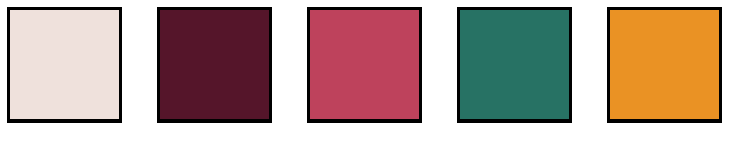
\includegraphics[height=1.25cm]{./graded-membership/figures/tarahumara-basic-categories.pdf}
  \caption[The basic colour categories for Central Tarahumara]{The
    basic colour categories for Central Tarahumara. These are the
    estimated foci of each category based on data from the World Color
    Survey \citep{kay10world}. From left to right (including the
    corresponding Munsell chip): \textit{ros\'a} (7.5R 9 2), \textit{ch\'o}
    (5.0R 2 8), \textit{sit\'a} (5.0R 5 14), \textit{siy\'o} (2.5BG 4 8) and
    \textit{sawar\'o} (5.0YR 7 14).}
  \label{f:gms-tarahumara-basic}
\end{figure}

As no exact data for the modifiers in Tarahumara are available, I have
estimated their prototypical membership values in such a way that each
of them cover a reasonable number of colour chips (560 for \textit{-kame},
1445 for \textit{-name} and 643 for \textit{-nanti}). Due to the absolute
nature of the membership categories, the proportion of the chips that
will be classified as each membership category depends on the colour
category they modify and its surrounding colour categories. The actual
prototypical values are provided in Table
\ref{t:gms-tarahumara-modifiers}.

\begin{table}[htpb]
  \centering
  \begin{tabular}{cd{4}}
  \lsptoprule
    membership category & \multicolumn{1}{c}{prototypical value}\\
    \midrule
    \itshape -kame & 0.2 \\
    \itshape -name & 0.02 \\
    \itshape -nanti & 0.002\\
    \lspbottomrule
  \end{tabular}
  \caption[Membership categories for Central Tarahumara]{Membership
    categories for Central Tarahumara. The higher the prototypical
    value, the more similar the colour category and the colour sample
    have to be.}
  \label{t:gms-tarahumara-modifiers}
\end{table}

A first test whether the proposed membership categories are valid is
provided by a naming benchmark\is{naming benchmark!for graded
  membership strategy}. This benchmark involves naming each of the
Munsell chips and grouping the samples based on the resulting
name. The results for two roots, \textit{sit\'a} and \textit{sawar\'o} are shown
in Figure \ref{f:gms-baseline-sita-sawaro}. In this figure, the
samples for one root are separated in more or less equal parts using
the three modifiers. These results are qualitatively similar to the
reported use of modifiers in Tamahumara as shown in Figure
\ref{f:gms-burgress-tarahumara}.

\begin{figure}[htbp]
\centering
\subfigure{
  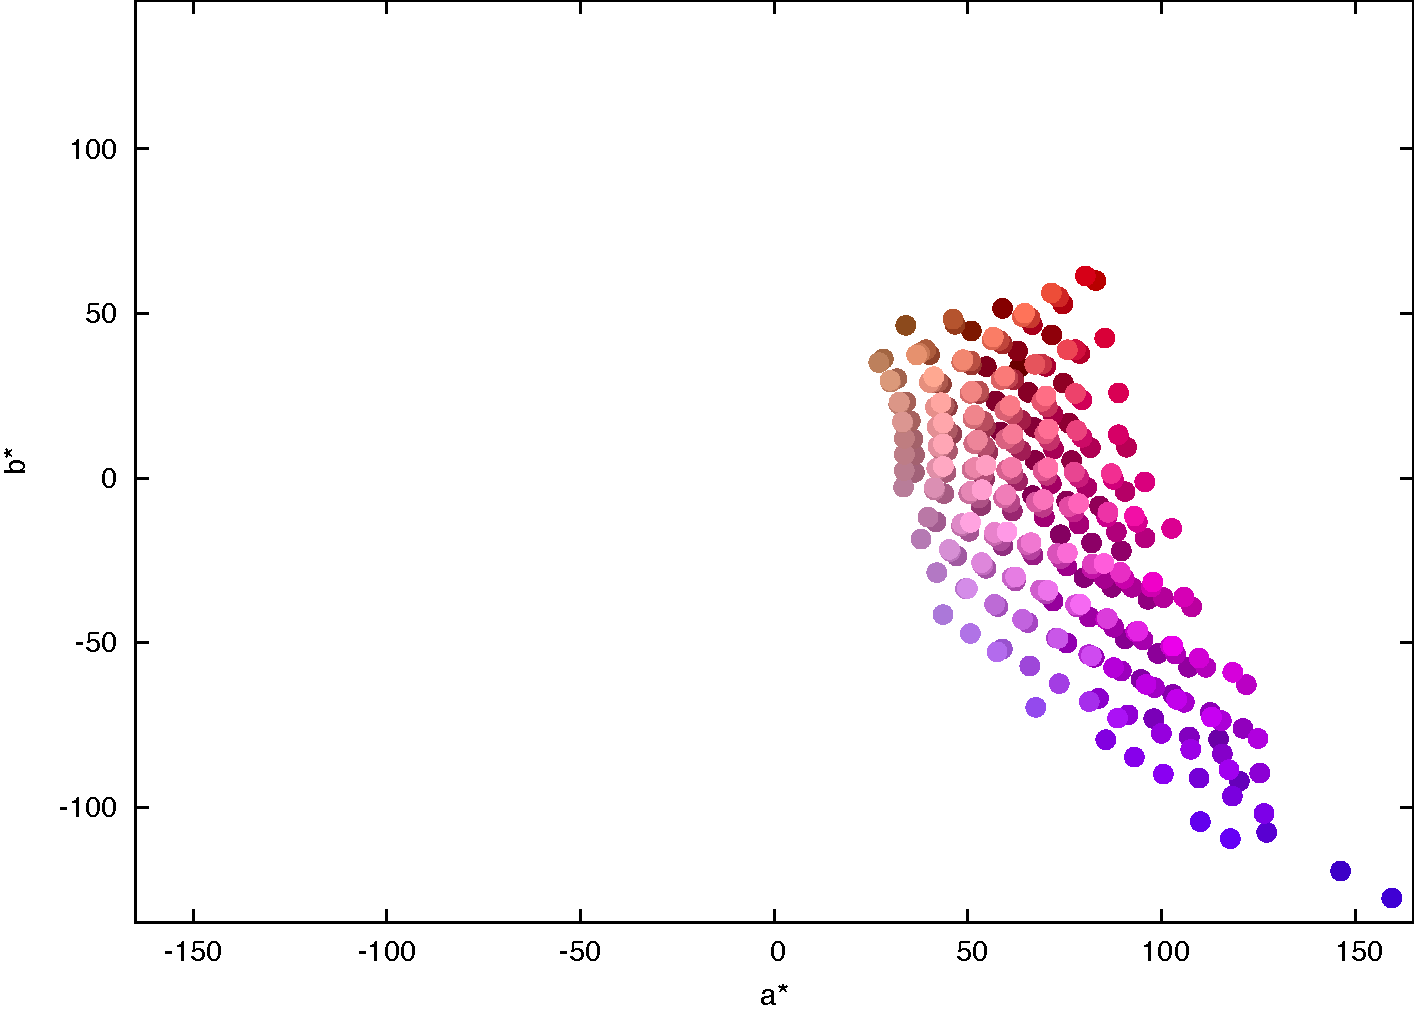
\includegraphics[width=.4\textwidth]{./graded-membership/figures/sita.pdf}
}
\subfigure{
  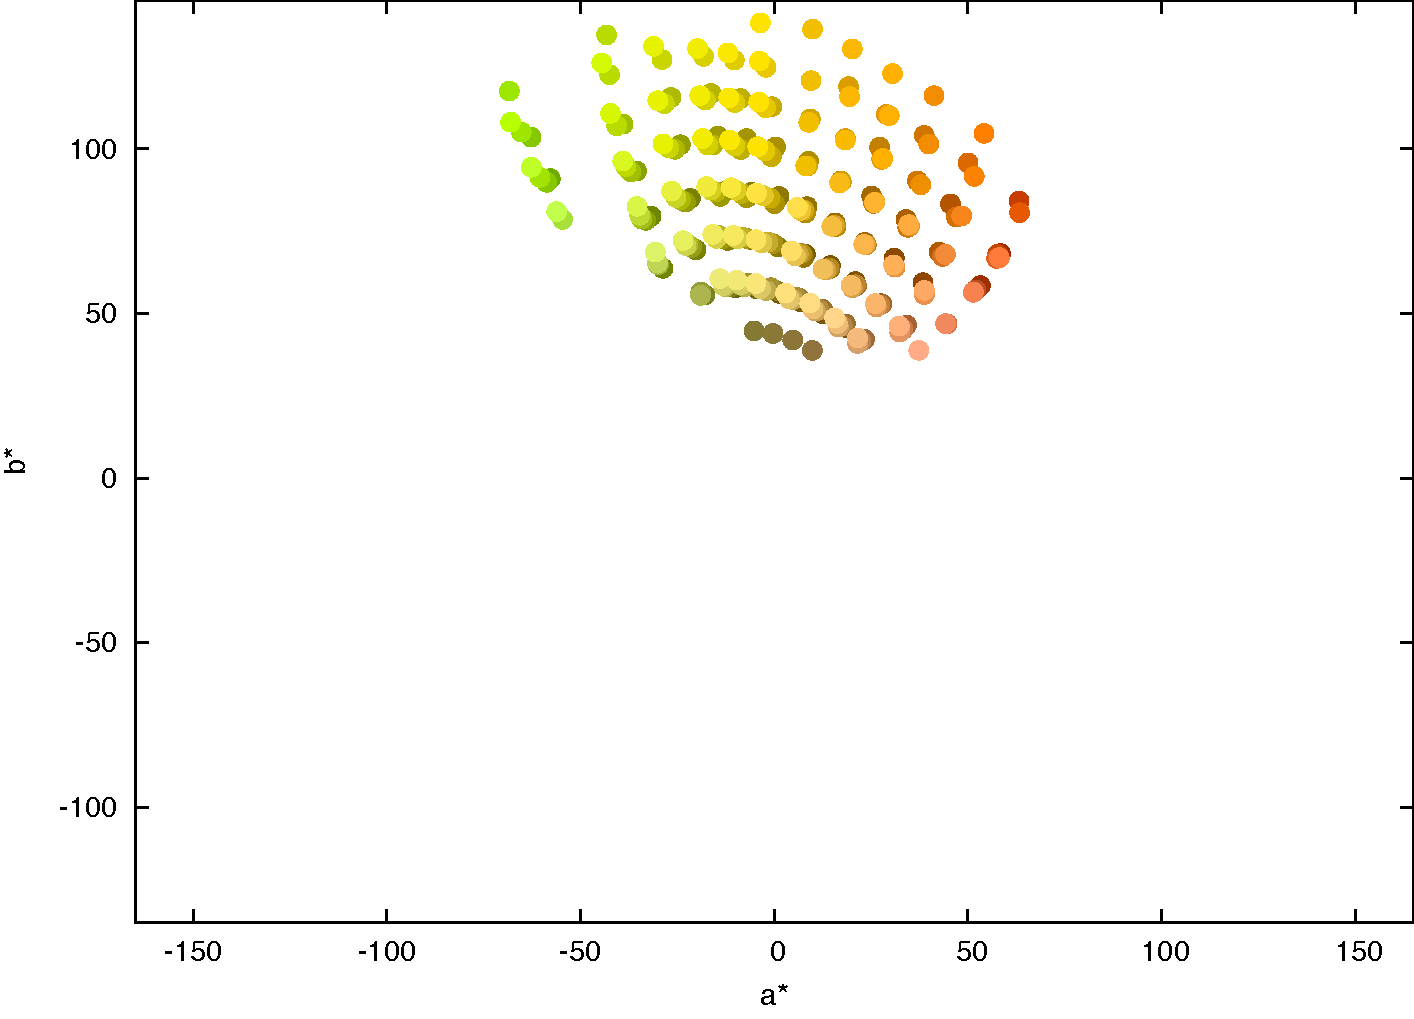
\includegraphics[width=.4\textwidth]{./graded-membership/figures/sawaro.pdf}
}
\subfigure{
  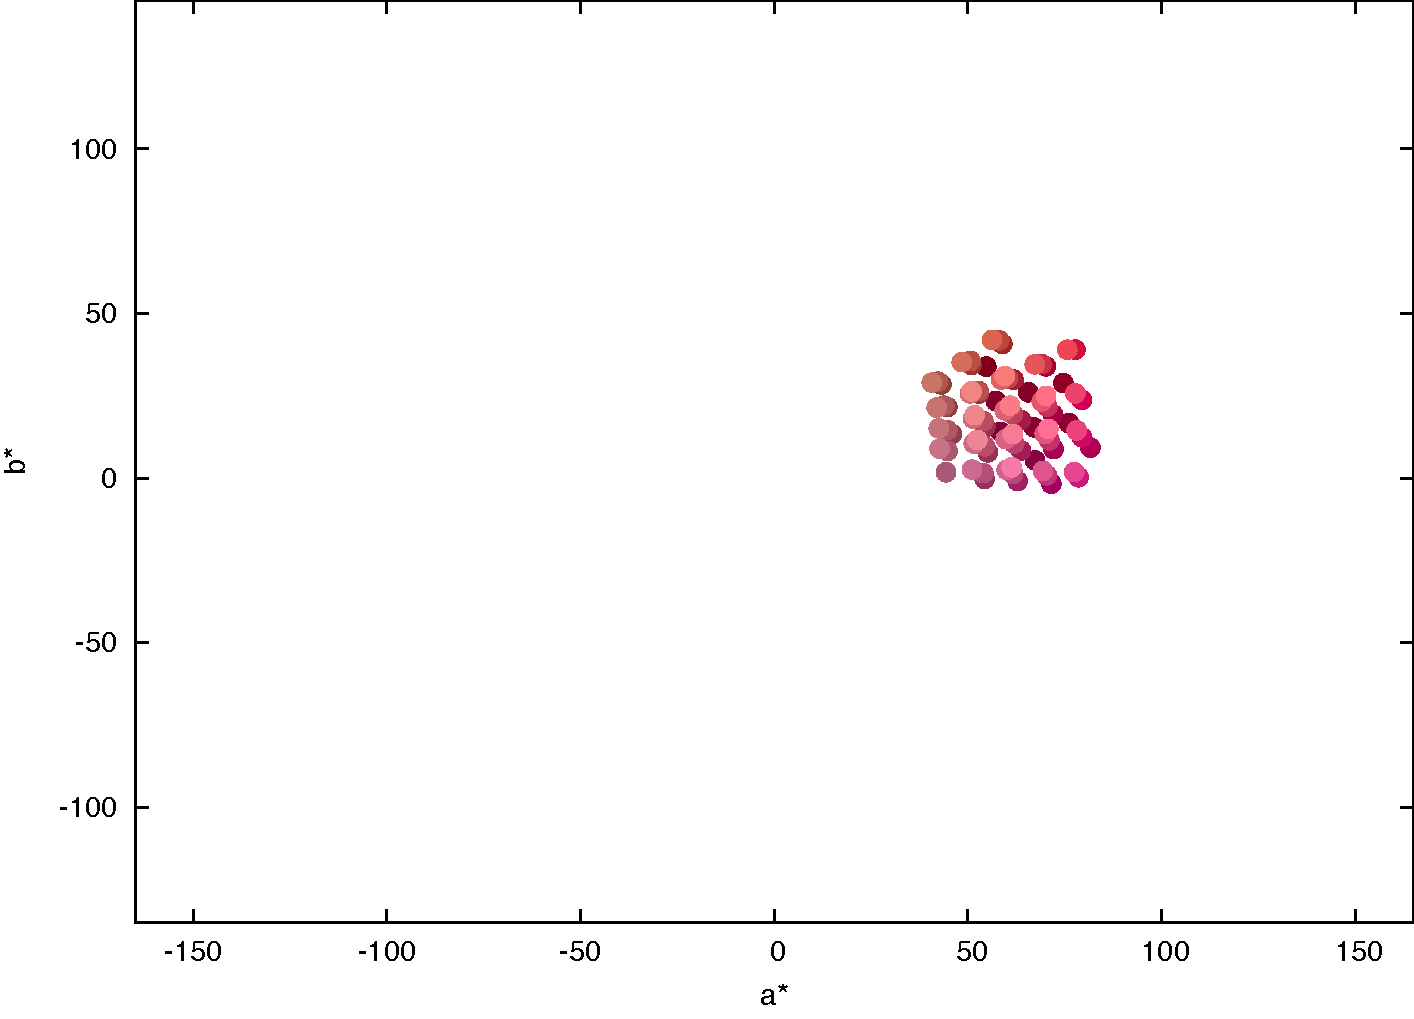
\includegraphics[width=.4\textwidth]{./graded-membership/figures/sita-kame.pdf}
}
\subfigure{
  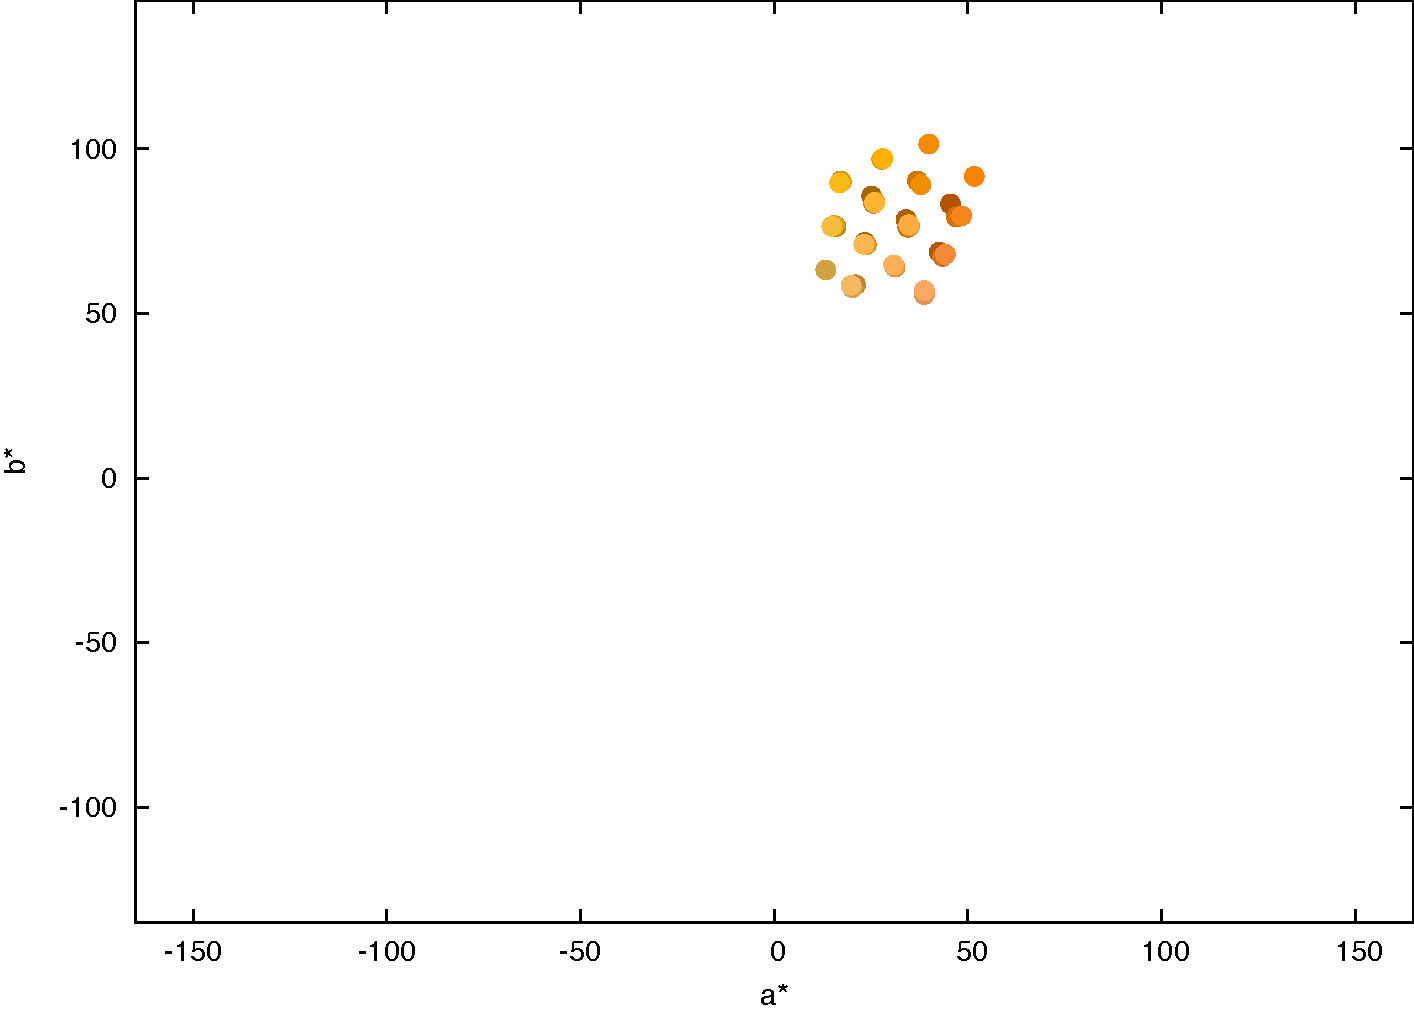
\includegraphics[width=.4\textwidth]{./graded-membership/figures/sawaro-kame.pdf}
}
\subfigure{
  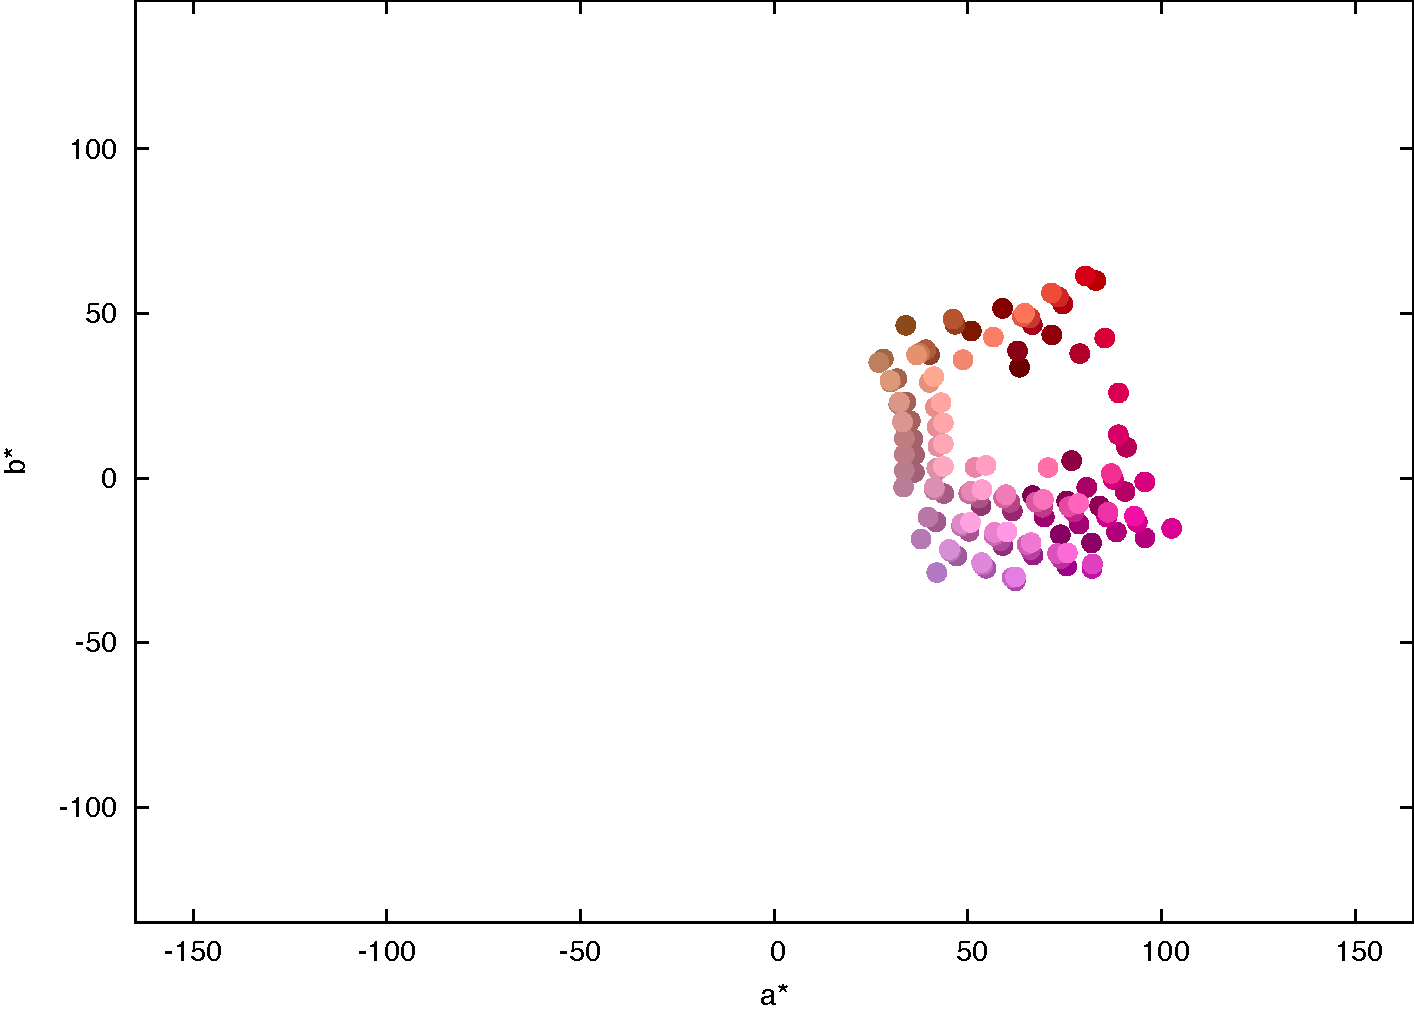
\includegraphics[width=.4\textwidth]{./graded-membership/figures/sita-name.pdf}
}
\subfigure{
  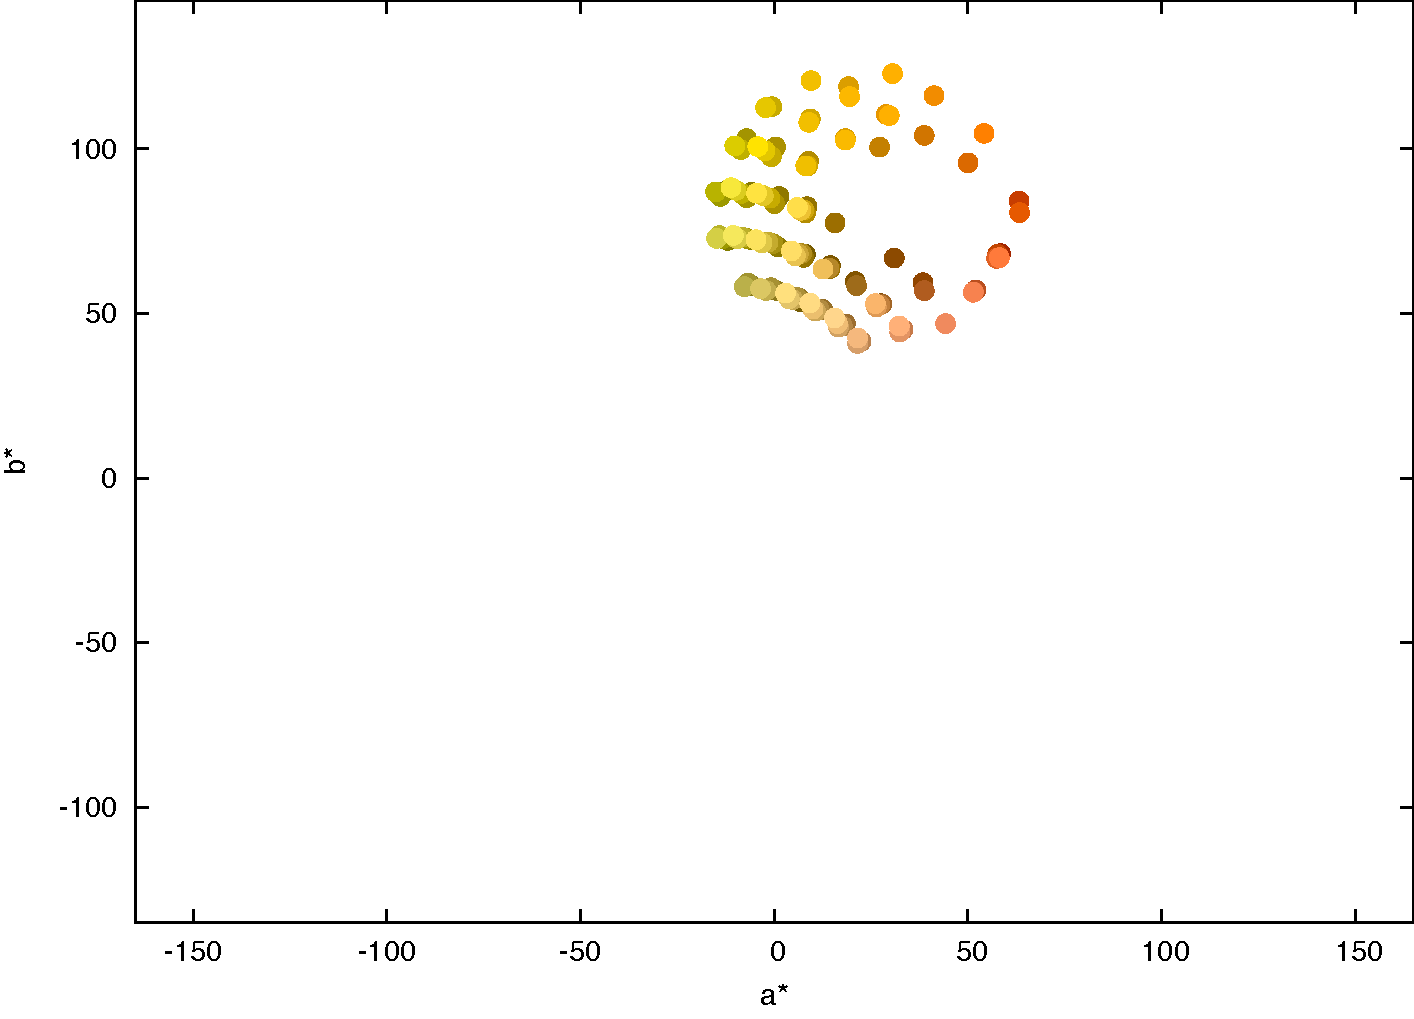
\includegraphics[width=.4\textwidth]{./graded-membership/figures/sawaro-name.pdf}
}
\subfigure{
  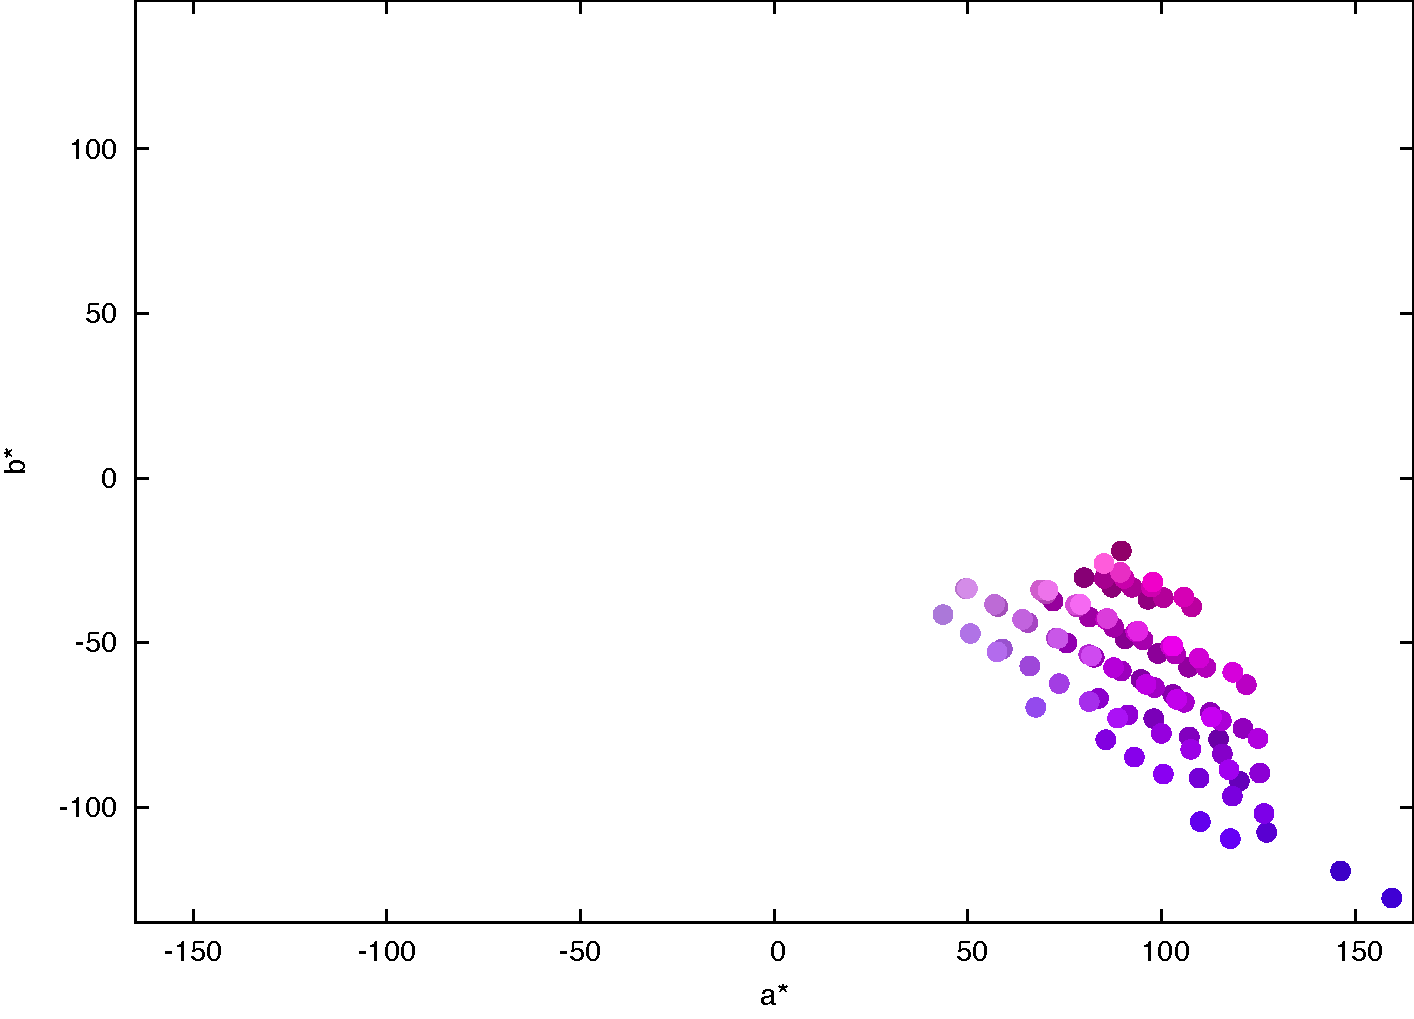
\includegraphics[width=.4\textwidth]{./graded-membership/figures/sita-nanti.pdf}
}
\subfigure{
  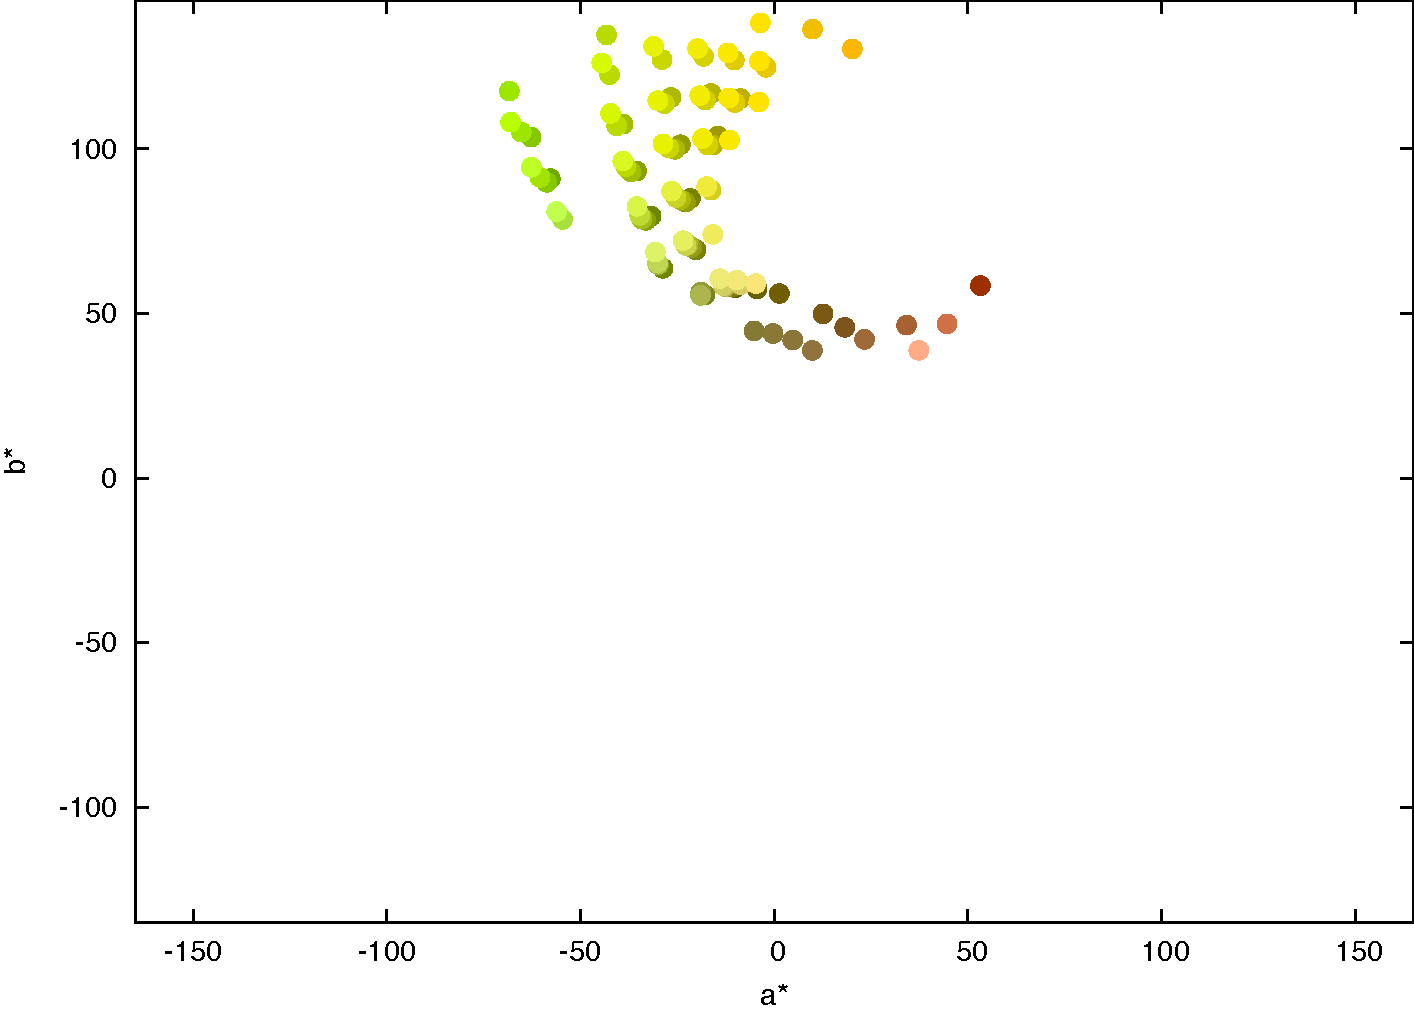
\includegraphics[width=.4\textwidth]{./graded-membership/figures/sawaro-nanti.pdf}
}
\caption[Example of modelled graded membership for Tarahumara]{Example
  of modelled graded membership for \textit{sit\'a} (`left') and \textit{sawar\'o}
  (`right') in Tamahumara. The top row shows the aggregate of all uses
  of the corresponding term as root , the second row the uses of the
  \mbox{\textit{-kame}} (`very') modifier, the third row the uses of \textit{-name}
  (`somewhat') and the bottom row show the uses of \textit{-nanti} (`only
  slightly'). All diagrams are projections on the hue plane of the CIE
  $L^*a^*b^*$ colour space.}
\label{f:gms-baseline-sita-sawaro}
\end{figure}

\begin{figure}
 \centering
  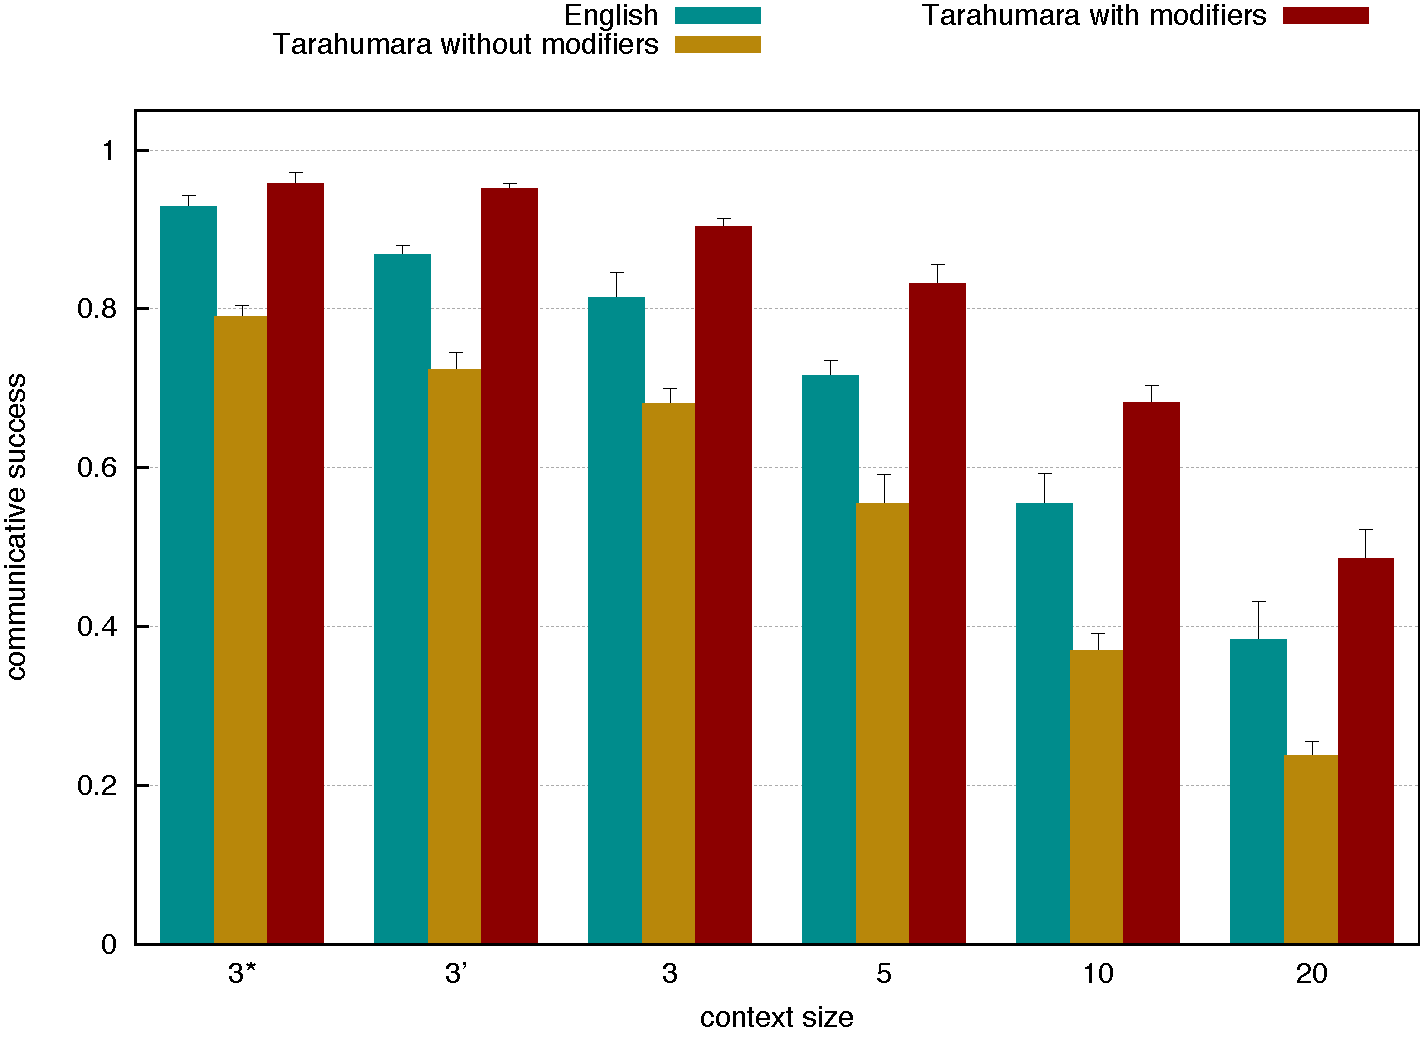
\includegraphics[width=.8\textwidth]{./graded-membership/figures/baseline.pdf}
  \caption[The baseline communicative success for graded membership
  strategy]{The baseline communicative success for graded membership
    strategy, comparing three different language systems: two are
    limited to the basic colour strategy and are based on English (11
    terms) and Tarahumara (5 terms). The third system is based on
    Tarahumara as well, but involves the graded strategy using 3
    modifiers. The lower number of basic terms has a negative impact
    on communicative success, but this can be overcome by allowing the
    use of modifiers.}
  \label{f:gms-baseline}
\end{figure}

\subsection{Results}
\label{s:gms-baseline-results}

The resulting communicative success of the baseline experiment is
shown in Figure \ref{f:gms-baseline}. A lower number of basic
categories has a negative impact on the communicative success (compare
English to Tarahumara without modifiers) but this effect can be
countered by allowing the use of modifiers (compare Tarahumara with
and without modifiers). Most interestingly, by allowing the use of
modifiers a system with a lower number of basic categories can become
more expressive than systems with a higher number of basic categories
that does not allow for modifiers (compare Tarahumara with modifiers
and English).

In systems in which only the strict basic strategy is deployed, the
chosen sample needs to be discriminable by one category which is
enforced by the selection process. The higher the number of
categories, the lower the chance another sample will be categorised as
the category of the topic. This explains the first observation that a
lower number of basic categories results in a lower baseline
communicative success.

When modifiers are allowed in the language system, the restriction of
a single discriminatory category is somewhat loosened. Instead of a
single category to be discriminative, it now is the consecutive
filtering using a colour category and a membership category that needs
to be discriminative. This explains why allowing modifiers has a
positive impact on the resulting baseline success.


\section{Conclusion}

In this chapter, I have introduced a compositional semantics for the
graded membership strategy and linguistic rules to express the
membership categories in language. I have qualitatively compared the
resulting names to those reported for the Tarahumara language using a
naming benchmark. I have also shown the positive impact of the use of
modifiers on the baseline communicative success, which can counter the
negative impact of a lower number of basic colour categories.